\subsection{\Mutex 和\RWMutex }
\begin{frame}{基本介绍}
    \begin{itemize}
        \item \Mutex 是``Mutual Exclusion''的缩写
        \item \textbf{用途}: 保护程序的\alert{关键区域}---需要排他地存取共享资源的程序片段
        \item \Mutex 和\RWMutex 要求开发者必须以\alert{特定的方式}访问内存以保证数据的同步
    \end{itemize}
\end{frame}

\begin{frame}[fragile]{示例}
\begin{lstlisting}[caption={\Mutex 使用示例}]
var count int
var lock sync.Mutex

increment := func() {
  lock.Lock()
  defer lock.Unlock()
  count++
  fmt.Printf("Incrementing: %d\n", count)
}
decrement := func() {
  lock.Lock() // 请求对关键区域--count变量的存取
  defer lock.Unlock()  // 放弃对关键区域的排他存取权利
  count--
  fmt.Printf("Decrementing: %d\n", count)
}
\end{lstlisting}
\end{frame}

\begin{frame}[fragile]{示例(续)}
    \begin{columns}[t]
        \begin{column}{0.5\textwidth}
\begin{lstlisting}[caption={\Mutex 使用示例(续)},firstnumber=last,xleftmargin=8pt]
// Increment
var arithmetic sync.WaitGroup
for i := 0; i <= 2; i++ {
  arithmetic.Add(1)
  go func() {
    defer arithmetic.Done()
    increment()
  }()
}
// Decrement
for i := 0; i <= 2; i++ {
  arithmetic.Add(1)
  go func() {
    defer arithmetic.Done()
\end{lstlisting}
        \end{column}
        \begin{column}{0.5\textwidth}
\begin{lstlisting}[caption={\Mutex 使用示例(续)},firstnumber=last,xleftmargin=8pt]
    decrement()
  }()
}
arithmetic.Wait()
fmt.Println("Arithmetic complete.")

// 输出:
// Decrementing: -1
// Incrementing: 0
// Incrementing: 1
// Decrementing: 0
// Decrementing: -1
// Incrementing: 0
// Arithmetic complete.
\end{lstlisting}
        \end{column}
    \end{columns}
\end{frame}

\begin{frame}{温馨提示}
    \begin{itemize}
        \item 锁\texttt{m}的\texttt{Lock()}调用之后应有配对的\texttt{defer m.UnLock()}语句
        \item \alert{进出关键区域的代价是昂贵的}
    \end{itemize}    
\end{frame}

\begin{frame}{读写锁\RWMutex }
    \alert{在写锁未被锁定之前},读写锁能够满足任意共存的读锁请求

    示例代码参见\href{https://github.com/sammyne/concurrency-in-go/blob/master/chapter03/sync.pkg/mutex/rwlock.go}{\Mutex 和\RWMutex 性能对比},具体结果如下图所示,\alert{可见,性能替身没有想象中的那么明显}

    \begin{figure}
        \centering
        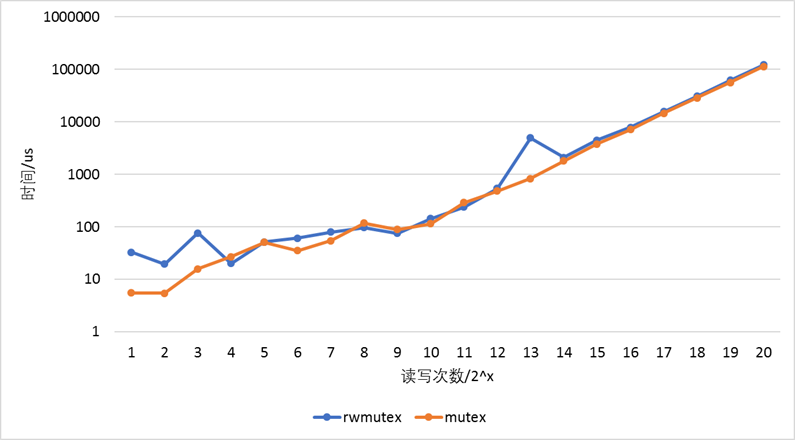
\includegraphics[width=0.7\textwidth]{images/rwmutex-vs-mutex.png}
        \caption{\Mutex 和\RWMutex 性能对比结果}
    \end{figure}
\end{frame}

\iffalse
\begin{frame}{读写锁\RWMutex }
    \alert{在写锁未被锁定之前},读写锁能够满足任意共存的读锁请求

    示例代码参见\href{https://github.com/sammyne/concurrency-in-go/blob/master/chapter03/sync.pkg/mutex/rwlock.go}{\Mutex 和\RWMutex 性能对比}

    程序的输出结果类似
    \begin{columns}
        \column{0.5\textwidth}
            \begin{table}
                \centering
                \caption{\Mutex 和\RWMutex 性能对比}
                \begin{tabular}{lll}
                    \hline
                    Readers  &RWMutex       &Mutex  \\
                    \hline
                    1        &32.87µs       &5.541µs \\
                    2        &19.603µs      &5.439µs \\
                    4        &76.62µs       &15.886µs \\
                    8        &20.201µs      &26.892µs \\
                    16       &51.558µs      &50.657µs \\
                    32       &61.313µs      &34.999µs \\
                    \hline
                \end{tabular}
            \end{table}

        \column{0.5\textwidth}
            \begin{table}
                \centering
                \caption{\Mutex 和\RWMutex 性能对比(续)}
                \begin{tabular}{lll}
                    \hline
                    Readers  &RWMutex       &Mutex  \\
                    \hline
                    64       &79.628µs      &54.763µs \\
                    128      &96.749µs      &118.701µs \\
                    256      &75.414µs      &89.375µs \\
                    512      &142.882µs     &114.705µs \\
                    1024     &239.471µs     &289.861µs \\
                    2048     &540.809µs     &479.173µs \\ 
                    \hline
                \end{tabular}
            \end{table}
    \end{columns}
\end{frame}

\begin{frame}{读写锁\RWMutex }
            \begin{table}[htbp!]
                \caption{\Mutex 和\RWMutex 性能对比(续)}
                \begin{tabular}{lll}
                    \hline
                    Readers  &RWMutex       &Mutex  \\
                    \hline
                    2048     &540.809µs     &479.173µs \\ 
                    4096     &4.982512ms    &827.095µs \\
                    8192     &2.09599ms     &1.790277ms \\
                    16384    &4.47045ms     &3.820926ms \\
                    32768    &7.911863ms    &7.163938ms \\
                    65536    &15.689641ms   &14.66057ms \\
                    131072   &31.016011ms   &28.674835ms \\
                    262144   &62.493129ms   &56.609731ms \\
                    524288   &121.927969ms  &113.786247ms \\   
                    \hline
                \end{tabular}
            \end{table} 
\end{frame}
\fi